\documentclass[../main.tex]{subfiles}
\usepackage{stmaryrd}





\begin{document}




\chapter{Oberts i tancats}






\section{Oberts i tancats}

\begin{defi}
[Obert]\label{def:obert}\index{Obert} Sigui $(X,\tau)$ un espai topològic. Es diuen \textit{oberts} als elements de la topologia.
\end{defi}

\begin{defi}
[Tancat]\label{def:tancattopologia}\index{Tancat (topologia)} Sigui $X$ un espai topològic. Un subconjunt $Z\subseteq X$ és \textit{tancat} si $X\setminus Z$ és obert.
\end{defi}

\begin{prop}
\label{prop:propietatstancatstopo} La col·lecció dels tancats d'un espai topològic satisfà:
\begin{enumerate}[(1)]
    \item Tant $\emptyset$ com $X$ són tancats.
    \item Si $\{Z_i\}_{i\in I}$ són tancats, aleshores $\bigcap_{i\in I}Z_i$ també és tancat.
    \item Si $Z_1,\ldots,Z_n$ són tancats de $X$, aleshores $Z_1\cup \cdots\cup Z_n$ també ho és.
\end{enumerate}
\end{prop}
\begin{proof}
\begin{enumerate}[(1)]
    \item Podem escriure $\emptyset = X\setminus X$ veient $X$ com un obert i $X = X\setminus \emptyset$, veient $\emptyset$ com un obert.
    \item En efecte,
    \begin{equation}
        \notag
        X\setminus\bigcap_{i\in I}Z_i = \bigcup_{i\in I}(X\setminus Z_i
    \end{equation}
    \item En efecte,
    \begin{equation}
        \notag
        X\setminus\left(\bigcup_{j=1}^nZ_j\right) = \bigcap_{j=1}^n(X\setminus Z_j).
    \end{equation}
\end{enumerate}
\end{proof}



De fet, en termes de la bijecció 
\begin{equation}
    \notag
    \begin{array}{rl}
        \{\text{oberts de $X$}\} & \longleftrightarrow \{\text{tancats de $X$}\}\\
        A & \longmapsto X\setminus A\\
        X\setminus Z & \longmapsfrom Z
    \end{array}
\end{equation}
les propietats (1), (2) i (3) es corresponen amb els axiomes (1), (2) i (3) respectivament, de la definició (\ref{def:topologia}) de topologia. Per tant, donat un conjunt $X$ i $\zeta\subseteq \mathscr{P}(X)$, els elements $\zeta$ són els tancats d'una topologia si i només si satisfan (1), (2) i (3) de (\ref{prop:propietatstancatstopo}).

Per tant, per descriure una topologia en un conjunt $X$ tenim dues possibilitats:
\begin{enumerate}[(i)]
    \item especificar els oberts $\tau\subseteq\mathscr{P}(X)$, que han de satisfer els axiomes (1), (2) i (3) de la definició (\ref{def:topologia}).
    \item especificar els tancats $\zeta\subseteq \mathscr{P}(X)$, que han de satisfer els axiomes (1), (2) i (3) de la proposició (\ref{prop:propietatstancatstopo}).
\end{enumerate}

\begin{ej}
\label{ej:obertsitancats1} Sigui $(X,\tau)$ un espai topològic. Aleshores $X$ i $\emptyset$ són oberts i tancats sempre. En efecte, clarament $\emptyset,X\in\tau$ per definició. Per tant $X,\emptyset$ són oberts. D'altra banda, $X\setminus X = \emptyset$ i $X\setminus \emptyset = X$, per tant també són tancats.
\end{ej}

\begin{ej}
\label{ej:obertsitancats2} Considerem $X = \{a,b,c\}$ i la topologia nidificada $\tau = \{\emptyset,\{a\},\{a,b\},X\}$. Aleshores $\emptyset,\{a\}$, $\{a,b\}$ i $X$ són oberts de $X$ i $\{b,c\}$ i $\{c\}$ són tancats (a més de $\emptyset,X$), ja que
\begin{equation}
    \notag
    \{b,c\} = X\setminus\{a\},\quad \text{i}\quad \{c\} = X\setminus\{a,b\}
\end{equation}
i $\{a\}$ i $\{a,b\}$ són oberts de $(X,\tau)$.
\end{ej}

\begin{ej}
\label{ej:obertsitancats3} Sigui $X = \{a,b,c,d\}$ i la topologia 
\begin{equation}
    \notag
    \tau = \{\emptyset,\{c\},\{a,b\},\{c,d\},\{a,b,c\},X\}
\end{equation}
Quins són els oberts i tancats de $X$ amb $\tau$?
\begin{itemize}
    \item Els oberts de $X$ són $\emptyset$, $\{c\}$, $\{a,b\}$, $\{c,d\}$, $\{a,b,c\}$ i $X$; és a dir, tots els elements de la topologia.
    \item Els tancats de $X$ són $X\setminus\{\text{oberts}\}$, és a dir
    \begin{equation}
        \notag
        X\setminus\{c\} = \{a,b,c\},\qquad X\setminus\{a,b\} = \{c,d\},\qquad X\setminus\{c,d\}=\{a,b\}
    \end{equation}
    \begin{equation}
        \notag
        X\setminus\{a,b,c\} = \{d\},\qquad X\setminus\emptyset = X,\qquad X\setminus X = \emptyset
    \end{equation}
\end{itemize}
Per tant, els que són oberts i tancats són $\emptyset, X$, $\{a,b\}$ i $\{c,d\}$.
\end{ej}

\begin{ej}
\label{ej:obertsitancats4} Trivialment, si $X$ està dotat de la topologia discreta $\tau = \mathscr{P}(X)$ aleshores tot subconjunt és obert de $X$. A més, si $A\subseteq X$, $A$ obert ergo $X\setminus A$ tancat. Però $X\setminus A\subseteq X$ i per tant també és obert i $A$ és tancat. Per tant, podem concloure que tot subconjunt és obert i tancat.
\end{ej}

\begin{ej}
\label{ej:obertsitancats5} Sigui $(\mathbb{Z},\tau_c)$ on $\tau_c$ és la topologia dels complements finits
\begin{equation}
    \notag
    \tau_c = \{U\subset\mathbb{Z}\;:\;\text{$U^c$ és finit}\}
\end{equation}
Estudiem si $2\mathbb{Z}=\{2n\;:\;n\in\mathbb{Z}\}\subseteq \mathbb{Z}$ és obert. Veiem que $2\mathbb{Z}^c$ és el conjunt dels enters senars, que és infinit. Així doncs, $2\mathbb{Z}\not\in\tau_c$ i $2\mathbb{Z}$ no és un obert. Altrament, $2\mathbb{Z}^c$ és el conjunt dels imparells que tampoc és obert ja que $(2\mathbb{Z}^c)^c = 2\mathbb{Z}$ tampoc no és finit. Així doncs no és ni obert ni tancat.
\end{ej}

\begin{ej}
\label{ej:obertsitancats6} Considerem l'espai topològic $(\mathbb{R},\tau)$, on $\tau = \{(-n,n)\;:\;n\in\mathbb{N}\}$. Quin és l'obert més gran contingut en $(-\pi,e)$? Demostrem també que tot subconjunt $A\subseteq X$ no trivial ($A\not=X,\emptyset$) no pot ser obert i tancat a l'hora.

Veiem que els oberts de $(\mathbb{R},\tau)$ són $(-1,1),(-2,2),\ldots$. Aleshores,
\begin{equation}
    \notag
    (-\pi,e)\approx (-3.141592..., 2.71828...)
\end{equation}
Per tant, l'obert més gran és $I_2 = (-2,2)\subseteq (-\pi,e)$. Podem veure clarament
\begin{equation}
    \notag
    (-1,1)\subset(-2,2)\subset(-\pi,e)
\end{equation}
però $(-3,3)\not\subset(-\pi,e)$ ja que $e<3$.

Suposem que $A$ és un obert. Aleshores $A = (-n,n)$ per algun $n\in\mathbb{N}$. Però $A$ no pot ser tancat ja que si $A$ és tancat, aleshores $A^c$ és obert i $A^c = (-\infty,-n)\cup (n,+\infty)\not\in\tau$.
\end{ej}

\begin{ej}
\label{ej:obertsitancats7} En general, si $(X,\tau)$ és un espai topològic, on $\tau$ és una topologia nidificada, no existeix cap obert i tancat no trivial. Vegem-ho:

Recordem que una topologia nidificada (\ref{def:topologianidificada}) era $\tau = \{U_1,U_2,\ldots\}$ de forma que $\emptyset\subset U_1\subset U_2\subset\cdots\subset X$. Suposem que $A\subset X$ és un obert no trivial. Si $A$ és obert, aleshores $\exists m_1\in\mathbb{N}$ tal que $A = U_{m_1}$. És a dir, que $U_1\subset U_2\subset\cdots\subset U_{m_1-1}\subset U_{m_1}$. Suposem que $A$ és també tancat. Aleshores $X\setminus A$ és obert, és a dir, existeix $m_2\in\mathbb{N}$ tal que $X\setminus A = U_{m_2}$. Aleshores $A\cap (X\setminus A) = \emptyset$, Sigui $M = \min\{m_1,m_2\}$. Aleshores, per la nidificació $U_{m_1}\cap U_{m_2} = U_M$ la qual cosa és una contradicció.
\end{ej}

\begin{ej}
\begin{enumerate}[(1)]
    \item Recordem que si $(X,d)$ és un espai mètric, $\forall x\in X$, $X\setminus\{x\}$ és un obert de la topologia discreta per $d$. Per tant $\{x\}$ és un tancat de $X$.
    \item Si $X$ té més d'un element, i dotem $X$ de la topologia grollera, els subconjunts de $X$ de la forma $\{x\}$ ($x\in X$ qualsevol) no són tancats.
\end{enumerate}
\end{ej}

\section{Punts interiors d'un conjunt en un espai topològic}

\subsection{Definició de punt interior i exemples}

\begin{defi}
[Punt interior]\label{def:puntinterior}\index{Punt interior}\index{Interior} Sigui $(X,\tau)$ un espai topològic i sigui $A\subseteq X$. Un punt $a\in X$ es diu \textit{punt interior} de $A$ si existeix un obert $U$ que contingui a $a$ tal que $a\in U\subseteq A$. El conjunt de tots els punts interiors d'$A$ es diu \textit{interior d'$A$} i s'escriu $A^{o}$.
\end{defi}

\begin{nota}
Per a qualsevol espai topològic $(X,\tau)$ se satisfà
\begin{enumerate}[(1)]
    \item $X^{o} = X$;
    \item $\emptyset^{o}=\emptyset$.
\end{enumerate}
\end{nota}
\begin{proof}
\begin{enumerate}[(1)]
    \item $X$ és obert. $\forall x\in X$, $X$ és un obert tal que $x\in X\subseteq X$, ergo $X^{o} = X$.
    \item $\emptyset$ obert. És trivial.
\end{enumerate}
\end{proof}

\begin{prop}
\label{prop:interior1} Sigui $(X,\tau)$ un espai topològic. Si $U\subseteq A\subseteq X$ i $U$ és un obert, aleshores $U\subseteq A^{o}$.
\end{prop}
\begin{proof}
Sigui $A$ un subconjunt de $X$ i $U$ un obert tal que $U\subseteq A\subseteq X$. Aleshores, $\forall a\in U$ tenim $a\in A$. Així, per cada $a\in A$, $U$ és un obert d'$A$ tal que $a\in U\subseteq A$, ergo $a\in A^{o}\Rightarrow U\subseteq A^{o}$.
\end{proof}

\begin{prop}
\label{prop:interior2} Sigui $(X,\tau)$ un espai topològic. Si $A\subseteq X$, aleshores $A^{o}$ és l'obert més gran contingut en $A$.
\end{prop}
\begin{proof}
Suposem que no. Aleshores, per algun $p\not\in A^{o}$, tenim $A^{o}\cup \{p\}$ és un obert més gran que $A^{o}$ contingut en $A$. Si $U = A^\circ\cup\{p\}\in\tau$ aleshores $p\in U=A^\circ\cup\{p\}\subseteq A$ i per definició $p\in A^\circ$ que és una contradicció.
\end{proof}

\begin{prop}
\label{prop:interior3} Sigui $(X,\tau)$ un espai topològic i $A\subseteq X$. Aleshores $(A^\circ)^\circ = A^\circ$.
\end{prop}
\begin{proof}
Per definició, $(A^\circ)^\circ$ és el conjunt de tots els punts interiors a $A^\circ$. Per la proposició (\ref{prop:interior1}), $A^\circ$ és obert i per tant tot punt de $A^\circ$ és un punt interior d'$A$. Per tant $A^\circ = (A^\circ)^\circ$ i per definició $(A^\circ)^\circ \subseteq A^\circ$.
\end{proof}

\begin{ej}
\label{ej:interior1} Considerem el conjunt $X = \{a,b,c\}$ amb la topologia nidificada $\tau = \{\emptyset,\{a\},\{a,b\},X\}$. Si prenem $A = \{a,c\}\subset X$, notem que $a\in A$ és punt interior d'$A$ ja que $U = \{a\}\in\tau$ i $a\in U\subseteq A$. Altrament, el punt $c\in A$ no és interior respecte $\tau$ perquè no existeix cap obert $U$ tal que $c\in U\subseteq A$. L'únic obert de $X$ que conté $c$ és $U = \{a,b,c\}$ i $U\not\subseteq A$. Així doncs, $A^\circ = \{a\}$.
\end{ej}

\begin{ej}
\label{ej:interior2} Considerem l'espai topològic $(\mathbb{R}^2,\tau)$, on $\tau$ és la topologia induïda per la mètrica estàndard $\|x-y\| = \sqrt{(x_1-y_1)^2+(x_2-y_2)^2}$ $\forall x = (x_1,x_2),y=(y_1,y_2)\in\mathbb{R}^2$. Un conjunt $S\subseteq \mathbb{R}^2$ és obert si i només si $\forall x\in S, \;\exists\varepsilon>0$ tal que $B(x,\varepsilon)\subseteq S$.\label{def:obertenespaieuclidia}

Sigui ara $A = [a,b)\times [c,d)\subseteq \mathbb{R}^2$. Gràficament:
\begin{equation}
    \notag
    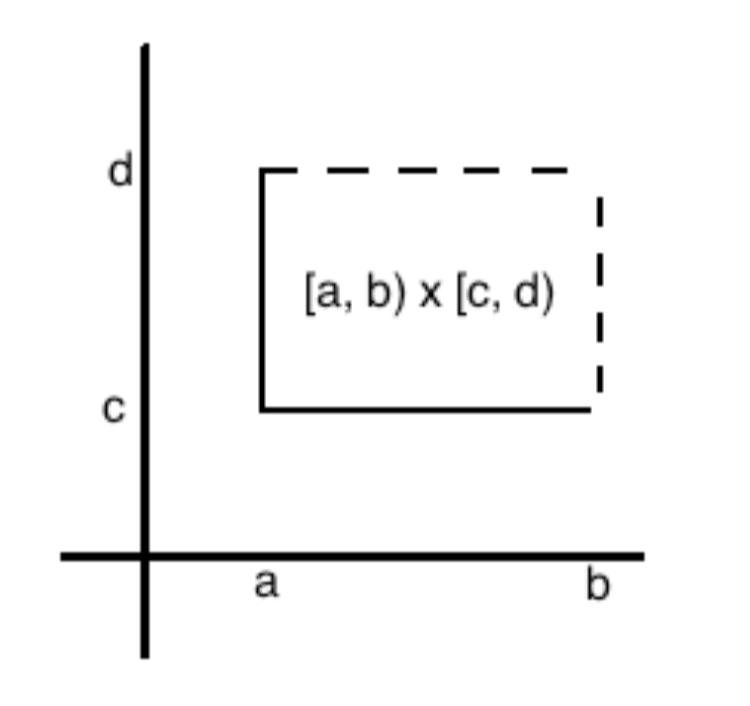
\includegraphics[scale = 0.2]{fotos_topo_1/interiorexemple1(1).jpeg}
\end{equation}
Els punts interiors a $A = [a,b)\times[c,d)$ són punts $x = (x_1,x_2)$ tals que $x_1\in (a,b)$ i $x_2\in (c,d)$. Qualsevol punt amb $x_1 = a$ i/o $x_2 = c$ no pot ser interior ja que no existiria cap real positiu $\varepsilon>0$ tal que la bola centrada en $x$ i de radi $\varepsilon$ estigués continguda en $A$, com s'il·lustra a la imatge.
\begin{equation}
    \notag
    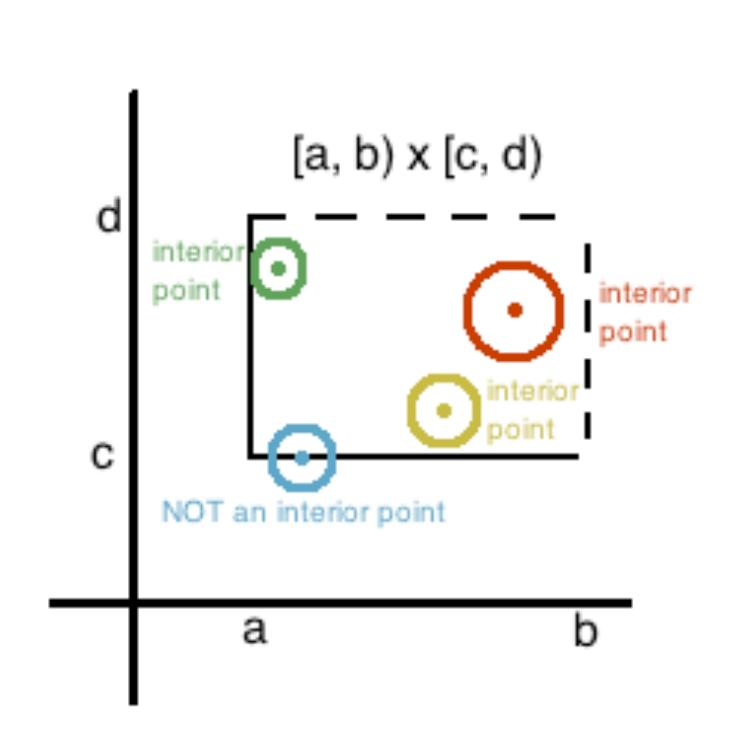
\includegraphics[scale = 0.2]{fotos_topo_1/interiorexemple1(2).jpeg}
    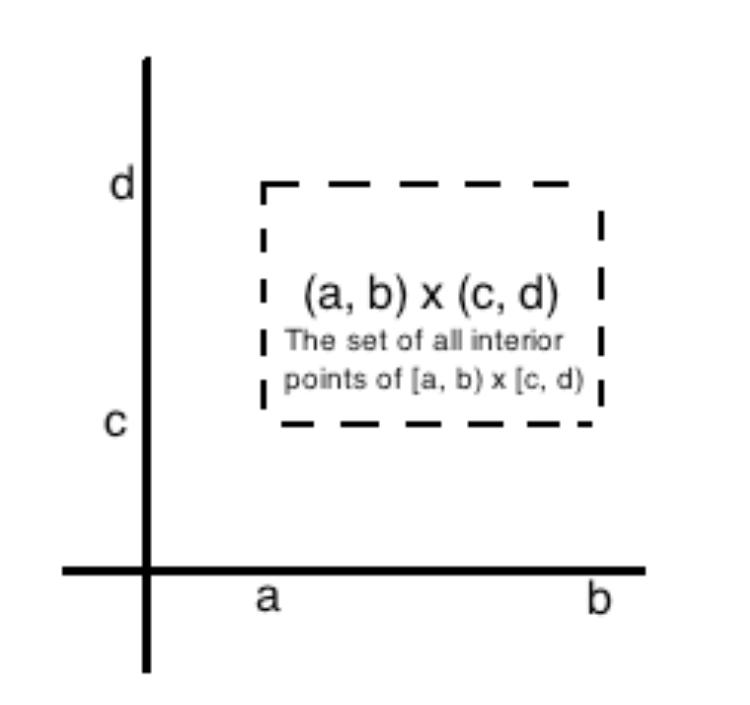
\includegraphics[scale = 0.2]{fotos_topo_1/interiorexemple1(3).jpeg}
\end{equation}
Així doncs, $A^\circ = (a,b)\times(c,d)$.
\end{ej}

\begin{ter}
\label{ter:interiorsiiobert} Sigui $(X,\tau)$ un espai topològic i sigui $A\subseteq X$. Aleshores $A$ és obert si i només si $A^\circ = A$, és a dir, si i només si tot punt d'$A$ és interior.
\end{ter}
\begin{proof}
Doble implicació.
\begin{enumerate}[($\Rightarrow$)]
    \item Suposem que $A$ és obert. Aleshores, $A\in\tau$ i per tot $a\in A$, podem prendre $U = A$ tal que $a\in U\subseteq A$. Per tant tot punt d'$A$ és interior i aleshores $A\subseteq A^\circ$. Com per definició $A^\circ\subseteq A$ ja tenim la igualtat.
\end{enumerate}
\begin{enumerate}[($\Leftarrow$)]
    \item Suposem $A = A^\circ$, és a dir, $\forall a\in A$, $a\in A^\circ$. Aleshores, $\forall a\in A$, $\exists U_a\in\tau$ tal que $a\in U_a\subseteq A$. Així, $A = \bigcup_{a\in A}U_a$ és obert ja que és la unió arbitrària d'oberts.
\end{enumerate}
\end{proof}

\begin{ej}
\label{ej:interior3} Considerem un conjunt arbitrari $X$ amb la topologia discreta $\tau = \mathscr{P}(X)$. Sigui $S\subseteq X$ un subconjunt de $X$. Què és l'interior de $S$?

Com $\tau$ és la topologia discreta, $S\in \tau$, ergo $S$ és obert i pel teorema (\ref{ter:interiorsiiobert}), agafem $U=S$ i $U$ satisfà $x\in U\subseteq S$, ergo $x\in S^\circ$. Així $S=S^\circ$.
\end{ej}

\begin{ej}
\label{ej:interior4} Sigui $(X,\tau_g)$ un espai topològic on $\tau_g = \{\emptyset, X\}$ és la topologia grollera. Sigui $S\subseteq X$. Quins són els punts interiors de $S$? Si $S\not=\emptyset$, aleshores $\emptyset\subseteq S\subseteq X$. $\forall x\in S$ veiem que $\nexists U\in \tau$ tal que $x\in U\subseteq S$. Per tant $S^\circ = \emptyset$.
\end{ej}

\begin{ej}
\label{ej:interior5} Considerem l'espai topològic $(X,\tau)$, on $\tau = \{(-n,n)\;:\;n\in\mathbb{N}\}$ i sigui $A = (-\pi,e)$. Recordant l'exemple (\ref{ej:obertsitancats6}) és fàcil veure que $(-\pi,e)^\circ = (-2,2)$.
\end{ej}

\begin{coro}
\label{coro:interior6} Sigui $(X,\tau)$ un espai topològic. Si $\forall A\subseteq X$ tenim $A^\circ = A$, aleshores $\tau$ és la topologia discreta. 
\end{coro}
\begin{proof}
Si $A = A^\circ$ $\forall A\subseteq X$ vol dir, pel teorema (\ref{ter:interiorsiiobert}), que tot subconjunt de $X$ és obert. Això vol dir: $\forall X\subseteq A$, $X\in\tau\Rightarrow \tau = \mathscr{P}(X)$.
\end{proof}

\subsection{Propietats}

\begin{prop}
\label{prop:propietat1interior} Sigui $(X,\tau)$ un espai topològic i $A,B\subseteq X$. Si $A\subseteq B$, aleshores $A^\circ\subseteq B^\circ$.
\end{prop}
\begin{proof}
Suposem $A\subseteq B$. Considerem $A^\circ$; sabem que és l'obert més gran contingut en $A$. En particular, $A^\circ\subseteq A\subseteq B$ i $A^\circ$ és doncs un obert contingut en $B$. Ara bé, $B^\circ$ és l'obert més gran contingut en $B$, per tant $A^\circ\subseteq B^\circ$.
\end{proof}

\begin{prop}
\label{prop:propietat2interior} Sigui $(X,\tau)$ un espai topològic i $A,B\subseteq X$. Aleshores, $A^\circ\cup B^\circ\subseteq (A\cup B)^\circ$.
\end{prop}
\begin{proof}
Sigui $x\in A^\circ\cup B^\circ$. Aleshores $x\in A^\circ$, o bé $x\in B^\circ$.

\begin{equation}
    \notag
    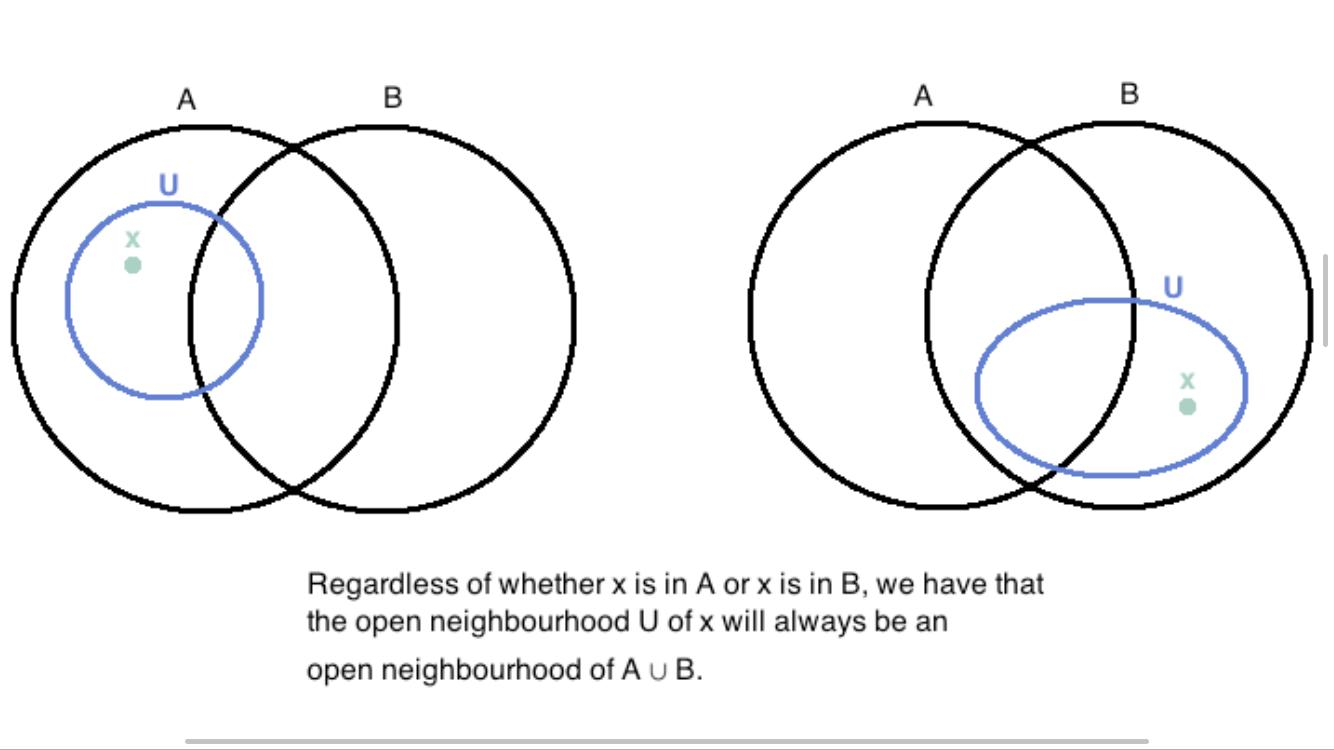
\includegraphics[scale = 0.2]{fotos_topo_1/interiorprop2.jpeg}
\end{equation}
Si $x\in A^\circ$, existeix un obert $U\in \tau$ tal que $x\in U\subseteq A$. Aleshores $x\in U\subseteq A\subseteq A\cup B$ i per tant $x\in (A\cup B)^\circ$. De la mateixa manera si $x\in B^\circ$ arribem a la mateixa conclusió.
\end{proof}

\begin{nota}
\label{nota:propietat2interior} En general $(A\cup B)^\circ\not\subseteq A^\circ\cup B^\circ$. Per exemple, si $A=(0,1]$ i $B=(1,2]$, aleshores $A^\circ = (0,1)$ i $B^\circ=(1,2)$ i $A^\circ\cup B^\circ = (0,1)\cup(1,2)$ mentre que $A\cup B=(0,2)$ i per tant $(A\cup B)^\circ = (0,2)$.
\end{nota}

Per veure un altre exemple d'això considerem $X = \{a,b,c,d\}$ amb la topologia donada per
\begin{equation}
    \notag
    \tau = \{\emptyset,\{b\},\{a,b\},\{b,c\},\{a,b,c\},X\}
\end{equation}
Considerem els conjunts $A = \{a\}$ i $B = \{b,c\}$. Clarament $A^\circ = \emptyset$ i $B^\circ = B$. Per tant, 
\begin{equation}
    \notag
    A^\circ\cup B^\circ = \emptyset\cup\{b,c\} = \{b,c\}
\end{equation}
D'altra banda, $A\cup B = \{a\}\cup\{b,c\} = \{a,b,c\}$ i $\{a,b,c\}^\circ = \{a,b,c\}\not\subseteq\{b,c\}$.

És per això que no tenim la igualtat a la proposició (\ref{prop:propietat2interior})

\begin{prop}
\label{prop:propietat3interior} Sigui $(X,\tau)$ un espai topològic i $A,B\subseteq X$. Aleshores $A^\circ\cap B^\circ = (A\cap B)^\circ$.
\end{prop}
\begin{proof}
Sigui $x\in A^\circ\cap B^\circ$. Aleshores $x\in A^\circ$ i $x\in B^\circ$. Per tant $\exists U_A\in\tau$ tal que $x\in U_A\subseteq A$ i $\exists U_B\in\tau$ tal que $x\in U_B\subseteq B$. Sigui $U = U_A\cap U_B$. Com la intersecció finita d'oberts és obert, $U\in \tau$ és un obert.
\begin{equation}
    \notag
    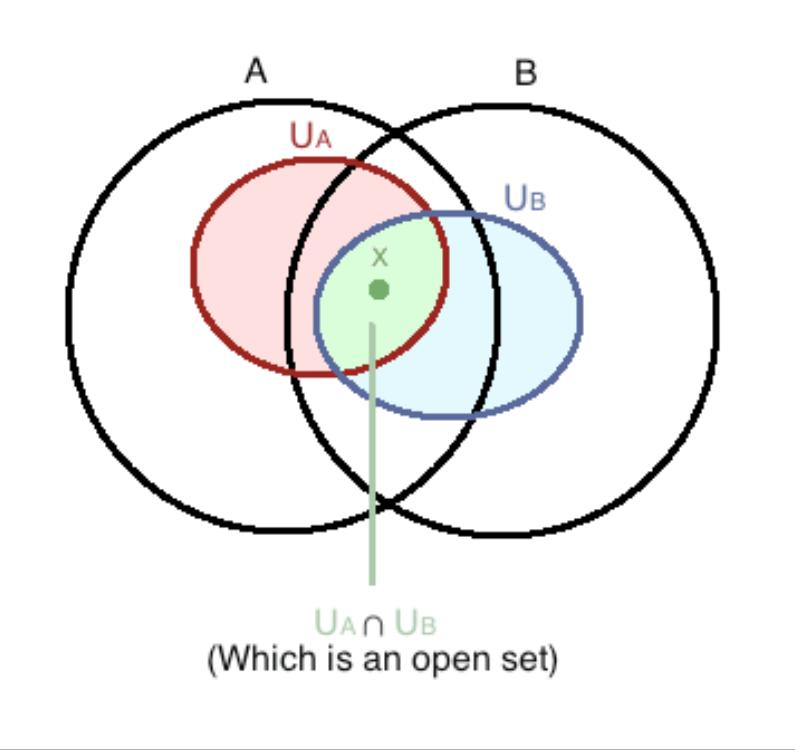
\includegraphics[scale = 0.2]{fotos_topo_1/interiorprop3(1).jpeg}
    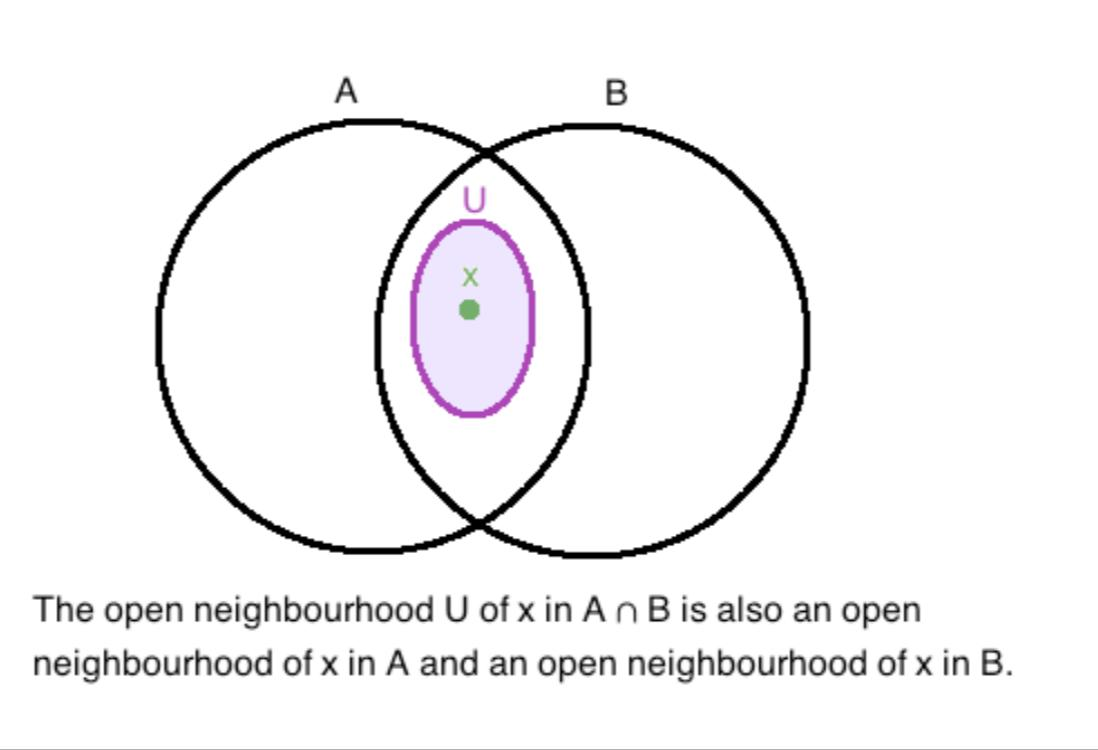
\includegraphics[scale = 0.2]{fotos_topo_1/interiorprop3(2).jpeg}
\end{equation}
Llavors $x\in U\subseteq A\cap B$ i això implica $x\in (A\cap B)^\circ$.

Sigui ara $x\in (A\cap B)^\circ$. Aleshores $\exists U\in\tau$ tal que $x\in U\subseteq A\cap B$. Però si $U\subseteq A\cap B$ aleshores $U\subseteq A$ i $U\subseteq B$, ergo $x\in U\subseteq A$ i $x\in U\subseteq B$ que implica que $x\in A^\circ$ i $x\in B^\circ$ per tant $x\in A^\circ\cap B^\circ$.
i amb això obtenim $(A\cap B)^\circ = A^\circ\cap B^\circ$ que ens dóna la igualtat.
\end{proof}

\section{Punts adherents d'un conjunt en un espai topològic}
\subsection{Definició de punt adherent o d'acumulació i exemples}

\begin{defi}
[Acumulació]\label{def:acumulacio}\index{Punt d'acumulació}\index{Acumulació} Sigui $(X,\tau)$ un espai topològic i sigui $A\subseteq X$. Un punt $x\in X$ es diu \textit{punt d'acumulació d'$A$} si tot obert contenint $x$ conté algun punt d'$A$ que no sigui $x$. És a dir, si $\forall U\in\tau$ tal que $x\in U$, $A\cap U\setminus\{x\}\not=\emptyset$. El conjunt de punts d'acumulació d'$A$ es denota per $A'$.
\end{defi}

Observem que un punt \underline{no} és d'acumulació si $\exists U\in\tau$ tal que $x\in U$ i $U\cap A\setminus \{x\}=\emptyset$. Això serà útil pels exercicis.

\begin{prop}
\label{prop:acumulacio1} Sigui $(X,\tau)$ un espai topològic i sigui $A\subseteq X$ un conjunt. Aleshores $A\cup A'$ és tancat.
\end{prop}
\begin{proof}
Sigui $x\in X\setminus (A\cup A')$. Aleshores $x\not\in A$ i $x\not\in A'$. Llavors $x$ no és d'acumulació d'$A$, cosa que implica que existeix un obert $U\ni x$ que no conté cap altre punt d'$A$ que no sigui $x$. Però també $x\not\in A$ llavors $U\cap A = \emptyset$. Com que aquest $U$ existeix per a cada $X\setminus(A\cup A')$ veiem que $X\setminus (A\cup A')$ és obert (perquè per a tot $x$ existeix $U\in\tau$ tal que $x\in U\subseteq X\setminus(A\cup A')$) i per tant $A\cup A'$ és tancat.
\end{proof}

\begin{ej}
\label{ej:acumulacio1} Considerem el conjunt finit $X = \{a,b,c\}$ i la topologia nidificada
\begin{equation}
    \notag
    \tau = \{\emptyset,\{a\},\{a,b\},\{a,b,c\}\}
\end{equation}
Sigui $A =X$. El punt $a\in X$ no és punt d'acumulació d'$A$ perquè l'obert $\{a\}\ni a$ no conté cap altre punt diferent d'$a$. D'altra banda, $b$ i $c$ sí són punts d'acumulació ja que tots els oberts contenint $b$ són $\{a,b\}$ i $\{a,b,c\}$ i tots compleixen
\begin{equation}
    \notag
    \{a,b\}\cap A \setminus\{b\} = \{a\}\not=\emptyset,\qquad \{a,b,c\}\cap A\setminus\{b\} = \{a,c\}\not=\emptyset
\end{equation}
i el mateix passa amb $c$. Així $A'=\{b,c\}$. Es pot comprovar que $A\cup A' = X$ és tancat.
\end{ej}

\begin{ej}
\label{ej:acumulacio2} Sigui $\mathbb{R}$ amb la topologia euclidiana. Sigui $A = (0,1)$. Aleshores tot $x\in A$ és un punt d'acumulació d'$A$. També 0 i 1 són punts d'acumulació d'$A$. De fet $A' = [0,1]$. En efecte, $\forall x\in [0,1]$ $\exists\varepsilon>0$ tal que $U_x = (x-\varepsilon,x+\varepsilon)$ és un obert contenint $x$ i tal que la seva intersecció amb $A$ conté més elements que $x$. Això prova que $[0,1]\subseteq A'$.
\end{ej}

\begin{ej}
\label{ej:acumulacio3} Considerem el conjunt dels reals $\mathbb{R}$ amb la topologia
\begin{equation}
    \notag
    \tau = \{\emptyset,X\}\cup\{(-n,n)\;:\;n\in\mathbb{N}\}
\end{equation}
Sigui $A = \mathbb{R}$. Considerem el punt $0\in\mathbb{R}$. Aleshores $(-1,1),(-2,2),\ldots\mathbb{R}$ són oberts que contenen al 0. Cadascun d'aquests oberts conté punts diferents del 0, per tant $0\in\mathbb{R}$ és un punt d'acumulació de $\mathbb{R}$ amb la topologia donada $\tau$.

Més enllà, tot punt $x\in \mathbb{R}$ és punt d'acumulació. Per veure això, fixem $x\in\mathbb{R}$. Aleshores $|x|>0$ i per la propietat arquimediana, existeix sempre $n_x\in\mathbb{N}$ tal que $|x|<n_x$. Així $-n_x<x<n_x$ i per la densitat dels nombres reals existeix $\xi\not=x$ tal que $-n_x<x<\xi<n_x$. Per tant, $\xi\in(-n_x,n_x)$. Tots els altres oberts més grans que aquest contenint $x$ són $(-n_x-k,n_x+k)$ amb $k\in\mathbb{N}$. A més, aquests oberts contenint $x$ estan nidificats
\begin{equation}
    \notag
    x,\xi\in (-n_x,n_x)\subset(-n_x-1,n_x+1)\subset\cdots\subset(-n_x-k,n_x+k)\subset\cdots
\end{equation}
Així doncs, per a cada obert contenint $x$ existeix $\xi\in\mathbb{R}$, $\xi\not=x$ contingut en cada interval. Llavors $x\in A'$.
\end{ej}

\begin{coro}
\label{coro:acumulacio4} Sigui $(X,\tau)$ un espai topològic i sigui $S\subseteq X$. Aleshores $\{x\}\in\tau$ si i només si $x$ no és punt d'acumulació de $S$.
\end{coro}
\begin{proof}
Suposem que $\{x\}\in\tau$. Aleshores $\{x\}$ és un obert contenint $x$. Però $\{x\}$ no conté cap altre punt de $S$ diferent de $x$. Per tant, $x\not\in S'$.

Recíprocament, suposem $x$ no és un punt d'acumulació de $S$. Aleshores existeix un entorn obert de $x$ que no conté cap altre punt diferent de $x$, és a dir, $\{x\}\in\tau$.
\end{proof}

\begin{ej}
\label{ej:acumulacio5} Sigui $(X,\tau)$ un espai topològic.
\begin{enumerate}[(1)]
    \item Si $\tau$ és la topologia discreta, no existeixen punts d'acumulació ja que $\{x\}$ és un obert contenint $x$ que no conté cap punt de $X$ diferent de $x$.
    \item Si $\tau$ és la topologia grollera, l'únic obert contenint $x\in X$ és $X$ per tot $x\in X$. Així doncs, $X$ conté elements de $X$ diferents de $x$ i aleshores si $X$ conté més d'un element, tot $x\in X$ és punt d'acumulació.
\end{enumerate}
\end{ej}

\subsection{Propietats}

\begin{prop}
\label{prop:propietat1acumulacio} Sigui $(X,\tau)$ un espai topològic i $A,B\subseteq X$. Aleshores, si $A\subseteq B$, llavors $A'\subseteq B'$.
\end{prop}
\begin{proof}
Suposem que $A\subseteq B$, i sigui $x\in A'$. Si $x$ és un punt d'acumulació de $A$, aleshores $\forall U\in\tau$ contenint $x$, se satisfà $A\cap U\setminus\{x\} \not=\emptyset$. Com $A\subseteq B$ veiem que $A\cap U\setminus\{x\}\subseteq B\cap U\setminus\{x\}$ i per tot $U\in\tau$ amb $x\in U$ tenim que $B\cap U\setminus\{x\}\not=\emptyset$ i això implica que $x\in B'$.
\end{proof}

\begin{prop}
\label{prop:propietat2acumulacio} Sigui $(X,\tau)$ un espai topològic i sigui $A,B\subseteq X$. Aleshores $A'\cup B'= (A\cup B)'$.
\end{prop}
\begin{proof}
Sigui $x\in A'\cup B'$. Aleshores $x\in A'$ o bé $x\in B'$. Si $x\in A'$, $x$ és un punt d'acumulació de $A$ i aleshores $\forall U\in\tau$ amb $x\in U$ tenim $U\cap A\setminus\{x\}\not=\emptyset$. Similarment, si $x\in B'$, $\forall U\in\tau$ tal que $x\in U$, $U\cap B\setminus\{x\}\not=\emptyset$. Ara:
\begin{equation}
    \notag
    [A\cap U\setminus\{x\}]\cup[B\cap U\setminus\{x\}] = (A\cup B)\cap U\setminus\{x\}\not=\emptyset
\end{equation}
És a dir, $\forall U\in\tau$ tal que $x\in U$ tenim que $(A\cup B)\cap (U\setminus\{x\})\not=\emptyset$, ergo $x\in (A\cup B)'$.

Sigui ara $x\in (A\cup B)'$. Suposem que $x\not\in A'\cup B'$. Aleshores, si $x\not\in A'$, $\exists U_A\in\tau$ tal que $x\in U_A$ i $U_A\cap A\setminus\{x\} = \emptyset$. Similarment, si $x\not\in B'$, $\exists U_B\in\tau$ tal que $x\in U_b$ i $B\cap U_B\setminus\{x\}=\emptyset$. Sigui ara $U = U_A\cup U_B$. Aleshores $x\in U$ i $(A\cup B)\cap U\setminus\{x\}=\emptyset$ cosa que contradiu que $x\in (A\cup B)'$.
\end{proof}

\begin{prop}
\label{prop:propietat3acumulació} Sigui $(X,\tau)$ un espai topològic i $A,B\subseteq X$. Aleshores $A'\cap B'=(A\cap B)'$.
\end{prop}
\begin{proof}
Sigui $x\in A'\cap B'$. Aleshores $x\in A'$ i $x\in B'$. Com $x\in A'$, $\forall U\in\tau$ tal que $x\in U$ tenim que $A\cap U\setminus\{x\}\not=\emptyset$. Similarment, com $x\in B'$, $\forall U\in\tau$ tal que $x\in U$ tenim $B\cap U\setminus\{x\}\not=\emptyset$. Així:
\begin{equation}
    \notag
    [A\cap U\setminus\{x\}]\cap[B\cap U\setminus\{x\}] = (A\cap B)\cap U\setminus\{x\} \not= \emptyset
\end{equation}
Per tant, $\forall U\in\tau$ tal que $x\in U$, $(A\cap B)\cap U\setminus\{x\}\not=\emptyset$ i això implica que $x\in (A\cap B)'$.

Recíprocament, suposem que $x\in (A\cap B)'$. Aleshores $\forall U\in\tau$ amb $x\in U$, tenim que $(A\cap B)\cap U\setminus\{x\}\not=\emptyset$. Aleshores, 
\begin{equation}
    \notag
    \emptyset\not= (A\cap B)\cap U\setminus\{x\} = [A\cap U\setminus\{x\}]\cap[B\cap U\setminus\{x\}]
\end{equation}
Com que la intersecció és no buida, aleshores cap dels dos conjunts és buit. Així $A\cap U\setminus\{x\}\not=\emptyset\not= B\cap U\setminus\{x\}$ i $x\in A'$ i $x\in B'$.
\end{proof}

\begin{ter}
\label{ter:tancatsiiacumulacio} Sigui $(X,\tau)$ un espai topològic i $A\subset X$. Aleshores $A$ és tancat si i només si $A$ conté tots els seus punts d'acumulació. És a dir, si i només si $A'\subseteq A$.
\end{ter}
\begin{proof}
Doble implicació
\begin{enumerate}[($\Rightarrow$)]
    \item Suposem $A$ tancat i suposem que no conté tots els punts d'acumulació. Aleshores $\exists x\in A'\setminus A$, ergo $x\in A^c=X\setminus A$.
    \begin{equation}
        \notag
        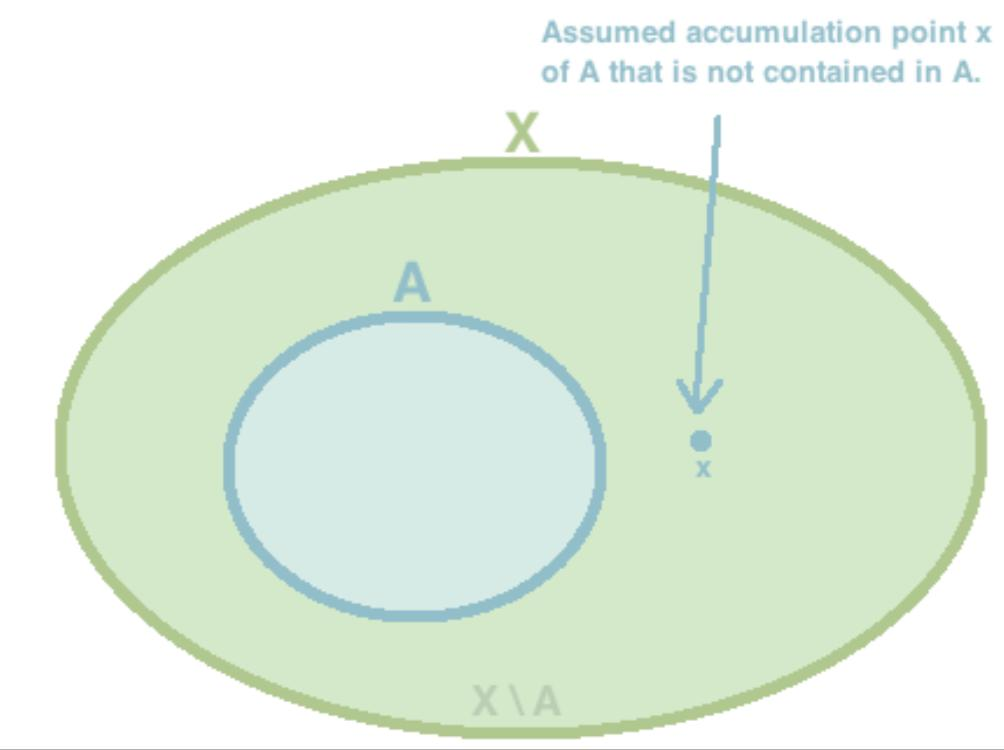
\includegraphics[scale = 0.2]{fotos_topo_1/teoremaacumulacio(1).jpeg}
    \end{equation}
    com $x$ és un punt d'acumulació d'$A$, per definició, tot obert $U\in\tau$ contenint $x$ conté també punts d'$A$ diferents de $x$.
    \begin{equation}
        \notag
        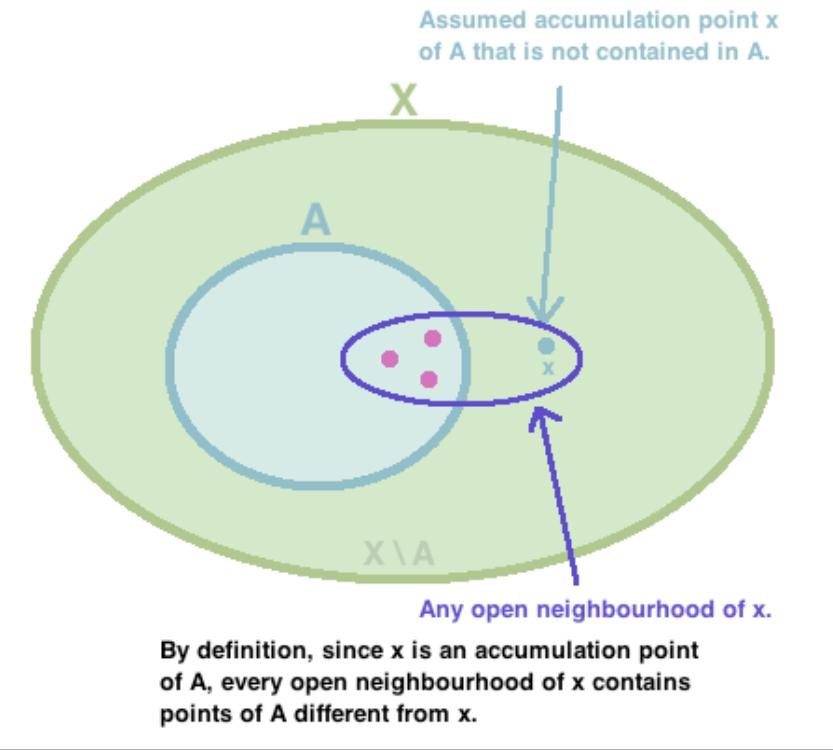
\includegraphics[scale = 0.2]{fotos_topo_1/teoremaacumulacio(2).jpeg}
    \end{equation}
    Per tant, no existeix cap obert $U$ tal que $x\in U\subseteq A^c = X\setminus A$ (ja que, si $x\in U$, aleshores $\exists a\in A$, $a\not=x$, tal que $a\in A$ i clarament $A\not\in A^c$).
    \begin{equation}
        \notag
        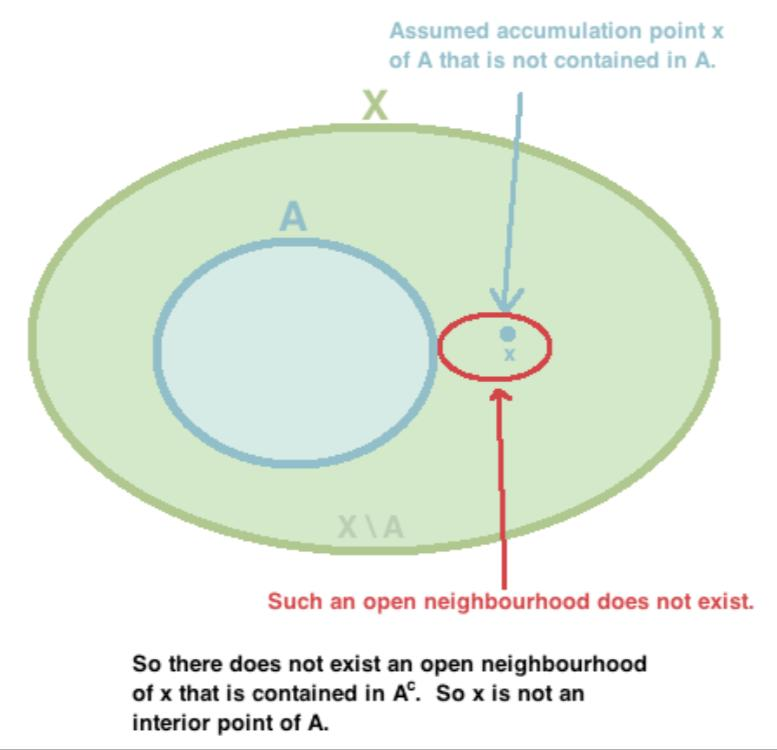
\includegraphics[scale = 0.2]{fotos_topo_1/teoremaacumulacio(3).jpeg}
    \end{equation}
    Així doncs, $x\not\in (A^c)^\circ$, ergo $(A^c)^\circ\not= A^c\Rightarrow A^c$ no és obert. Contradicció. Aleshores és absurd suposar que no conté tots els punts d'acumulació
\end{enumerate}
\begin{enumerate}[($\Leftarrow$)]
    \item Suposem ara que $A$ conté tots els punts d'acumulació d'$A$. Hem de veure que $A$ és tancat o, equivalentment, que $A^c$ és obert. $A^c$ és obert $\Leftrightarrow (A^c)^\circ = A^c$ pel teorema (\ref{ter:interiorsiiobert}). Sigui $x\in A^c$, com $A$ conté tots els punts d'acumulació, $x$ no pot ser d'acumulació, ergo $\exists U\in \tau$ obert contenint $x$ tal que $A\cap U\setminus\{x\}=\emptyset$. Però $x\not\in A$ ja que $x\in A^c$, així $U\subseteq A^c$ que implica que $x\in (A^c)^\circ$, així $A^c = (A^c)^\circ$ (ja que l'altra inclusió és trivial) i $A^c$ és obert, per tant $A$ és tancat.
\end{enumerate}
\end{proof}

\section{Clausura d'un conjunt en un espai topològic}
\subsection{Clausura d'un conjunt en un espai topològic}

\begin{defi}[Clausura]
\label{def:clausura}\index{Clausura} Sigui $(X,\tau)$ un espai topològic i $A\subseteq X$. La \textit{clausura} d'$A$ és el tancat més petit contenint $A$. S'escriu $\overline{A}$.
\end{defi}

Equivalentment podem dir que la clausura de $A$ és la intersecció de tots els tancats de $X$ que contenen $A$:
\begin{equation}
    \notag
    \overline{A} = \bigcup_{\substack{T\subseteq X\;\text{tancat}\\ A\subseteq T}} T
\end{equation}

\begin{prop}
\label{prop:clausura1} Sigui $(X,\tau)$ un espai topològic qualsevol. Aleshores $\overline{\emptyset} = \emptyset$ i $\overline{X}=X$.
\end{prop}
\begin{proof}
Per definició $\emptyset, X$ són tancats.
\end{proof}

\begin{prop}
\label{prop:clausura2} Sigui $(X,\tau)$ un espai topològic i $A\subseteq X$. Aleshores $\overline{\overline{A}} = \overline{A}$
\end{prop}
\begin{proof}
Per definició, $\overline{\overline{A}}$ és el tancat més petit contenint $\overline{A}$, però $\overline{A}$ ja és un tancat contenint-se a ell mateix i n'és el més petit, ergo $\overline{\overline{A}} = \overline{A}$.
\end{proof}

\begin{prop}
\label{prop:clausura3} Sigui $(X,\tau)$ un espai topològic i $A\subseteq X$. Aleshores $a\in \overline{A}$ si i només si $U\cap A\not=\emptyset$ per tot obert $U$ contenint $a$.
\end{prop}
\begin{proof}
Doble implicació.
\begin{enumerate}[($\Rightarrow$)]
    \item Sigui $a\in \overline{A}$, suposem que existeix un obert $U\ni a$ tal que $A\cap U=\emptyset$. Aleshores $A\subset X\setminus U$. Ara, com $U$ és obert, $X\setminus U$ és tancat i $A\subset X\setminus U$. Però $\overline{A}$ és el tancat més petit que conté a $A$. Ergo $\overline{A}\subset X\setminus U$. Però això no pot ser ja que $a\in \overline{A}$ i $a\in U\Rightarrow A\not\in X\setminus U$. Per tant, ha de ser $\forall U\ni a$, $U\cap A\not=\emptyset$.
\end{enumerate}
\begin{enumerate}[($\Leftarrow$)]
    \item Suposem ara que $U\cap A\not=\emptyset$ $\forall U\in\tau$ amb $a\in U$. Si $a\not\in\overline{A}$ aleshores $a\in X\setminus \overline{A}$. Però $X\setminus \overline{A}$ és un obert contenint $a$ i per tant $(X\setminus \overline{A})\cap A\not=\emptyset$ cosa impossible ja que $A\subseteq\overline{A}$ per definició.
\end{enumerate}
\end{proof}

\begin{ej}
\label{ej:clausura1} Considerem l'espai topològic $(\mathbb{R},\tau)$ on $\tau$ és la topologia usual (euclidiana), i sigui $A=[0,1)$. Què és $\overline{A}$? Veiem que $\overline{A} = [0,1]$. Per veure això hem de veure que és tancat i que n'és el més petit contenint $A$. Tancat és clar ja que $X\setminus[0,1] = (-\infty,0)\cup(1,+\infty)$ i tots dos són oberts de $\tau_e$.A més, $\nexists$ interval tancat més petit que $[0,1]$ contenint $[0,1)$.
\end{ej}

\begin{ej}
\label{ej:clausura2} Considerem $X = \{a,b,c,d\}$ i la topologia
\begin{equation}
    \notag
    \tau = \{\emptyset,\{b\},\{a,b\},\{b,c\},\{a,b,c\},X\}
\end{equation}
Sigui $A = \{b,d\}$. Quina és la clausura d'$A$? Primer estudiem els tancats de $X$ que són els complementaris dels elements de $\tau$:
\begin{equation}
    \notag
    \emptyset,\{d\},\{a,d\},\{c,d\},\{a,c,d\}, X
\end{equation}
Ara es tracta de trobar el tancat més petit que contingui a $\{b,d\}$. Aquest és $X$, per tant $\overline{A} = X$. Si en comptes considerem $B = \{a\}$, fàcilment es veu $\overline{B} = \{a,d\}$.
\end{ej}

\begin{ej}
\label{ej:clausura3} Considerem l'espai topològic $(X,\tau_d)$ on $\tau_d$ és la topologia discreta. Quina és la clausura de $A\subseteq X$? Recordem que amb la topologia discreta, tot subconjunt de $X$ és obert i per extensió, tot subconjunt de $X$ és tancat. Així doncs, $\forall A\subseteq X$, $\overline{A} = A$.
\end{ej}

\begin{ej}
\label{ej:clausura4} Considerem l'espai topològic $(X,\tau_g)$, on $\tau_g = \{\emptyset, X\}$ és la topologia grollera. Els únics tancats són, doncs $\emptyset$ i $X$. Per tant, $\forall A\not=\emptyset$, $A\subseteq X$, tenim $\overline{A} = X$; a més $\overline{\emptyset}= \emptyset$.
\end{ej}

\begin{ej}
\label{ej:clausura5} Considerem l'espai topològic $(\mathbb{R},\tau)$, amb
\begin{equation}
    \notag
    \tau = \{\emptyset, X\}\cup\{(-n,n)\;:\;n\in\mathbb{N}\}
\end{equation}
Siguin $A = \{0\}$ i $B = (2,3)$. Quines són les seves clausures? Notem que els oberts de $\mathbb{R}$ amb $\tau$ són $(-1,1)$, $(-2,2)$,$\ldots$. Aleshores, els tancats de $X$ seran
\begin{equation}
    \notag
    (-\infty,-1]\cup[1,+\infty),(-\infty,-2]\cup[2,+\infty),\ldots 
\end{equation}
Notem que cap d'aquests tancats conté el 0, excepte $\mathbb{R}$. Així doncs, $\overline{\{0\}}=\mathbb{R}$. D'altra banda veiem que $(2,3)\subseteq(-\infty,-2)\cup[2,+\infty)$ i així aquest és la seva clausura.
\end{ej}

\begin{ej}
\label{ej:clausura6} Considerem l'espai topològic $(\mathbb{N},\tau)$ on $\tau$ és la topologia dels complements finits. Sigui $A = \{1,2,3\}$. Quina és la clausura de $A$? I sigui $E = 2\mathbb{Z}$, quina és la seva clausura? Veiem que els oberts són aquells els complementaris dels quals són finits, així doncs, els tancats són tots els conjunts finits, ja que si $\{a_1,a_2,\ldots,a_k\}$ és finit, $\mathbb{N}\setminus\{a_1,\ldots,a_k\}$ és un obert de $(\mathbb{N},\tau)$ i per tant $\{a_1,\ldots,a_k\}$ és tancat. Així doncs, $A = \overline{A}$ ja que $A$ és finit. D'altra banda, $E$ infinit, i el seu complementari és el conjunt dels nombres senars, que també és infinit. Per tant, $\overline{E} = \mathbb{N}$.
\end{ej}

\subsection{Propietats}

\begin{ter}
\label{ter:clausuraigualaadherenciaunioconjunt} Sigui $(X,\tau)$ un espai topològic i $A\subseteq X$. Se satisfà $\overline{A} = A'\cup A$.
\end{ter}
\begin{proof}
Sigui $x\in \overline{A}$. Aleshores, $x$ està contingut en el tancat més petit que conté a $A$. Així, $x\in A$ o bé $x\in \overline{A}\setminus A$. Si $x\in A$ ja tenim $x\in A\cup A'$. Si $x\in\overline{A}\setminus A$, $x\not\in A$ i aleshores $x\not\in A^\circ$. Així doncs, $\nexists U$ obert tal que $x\in U$ satisfent $x\in U\subseteq A$. Aleshores, $\forall U\in\tau$ amb $x\in U$ tenim que
\begin{equation}
    \notag
    A\cap U = A\cap U\setminus\{x\} \not=\emptyset
\end{equation}
i per tant $x\in A'$. Així tenim $x\in A\cup A'$, és a dir $\overline{A}\subseteq A\cup A'$.

Recíprocament, suposem $x\in A\cup A'$. Si $x\in A$ ja hem acabat perquè $A\subseteq \overline{A}\Rightarrow x\in \overline{A}$. Suposem que $x\not\in A$ i $x\in A'\setminus A$. Aleshores $x$ és un punt d'acumulació i $\forall U\in\tau$ contenint $x$, $A\cap (U\setminus\{x\})\not=\emptyset$. Com $A\subseteq \overline{A}$, tenim doncs que $\forall U\in\tau$ tal que $x\in U$, $\overline{A}\cap U\setminus\{x\}\not=\emptyset$ i aleshores $x$ és un punt d'acumulació d'$\overline{A}$. Però $\overline{A}$ és tancat i pel teorema (\ref{ter:tancatsiiacumulacio}) $\overline{A}$ conté tots els punts d'acumulació ($\overline{A} = (\overline{A})'$). Així, $x\in \overline{A}$. Amb això $A\cup A'\subseteq\overline{A}$ i ja tenim la igualtat.
\end{proof}

\begin{ter}
\label{ter:tancatsiiclausura} Sigui $(X,\tau)$ un espai topològic i $A\subseteq X$. Aleshores, $A$ és tancat si i només si $\overline{A} = A$.
\end{ter}
\begin{proof}
Suposem que $A$ és tancat. Aleshores $\overline{A}=A$ ja que $A$ és el tancat més petit contenint $A$. Recíprocament, si $\overline{A} = A$, com $\overline{A}$ és tancat per definició, $A$ també ho és.
\end{proof}

\begin{prop}
\label{prop:propietat1clausura} Sigui $(X,\tau)$ un espai topològic i $A,B\subseteq X$. Si $A\subseteq B$, aleshores $\overline{A}\subseteq \overline{B}$.
\end{prop}
\begin{proof}
Suposem $A\subseteq B$. Sigui $x\in\overline{A}$. Com $\overline{A} = A\cup A'$ pel teorema (\ref{ter:clausuraigualaadherenciaunioconjunt}) tenim $x\in A\cup A'$ que implica que $x\in A$ o bé $x\in A'$. Si $x\in A$ com $A\subseteq B$, $x\in B$ i $x\in B\cup B'$. Si $x\in A'$ ja hem provat que $A'\subseteq B'$ en (\ref{prop:propietat1acumulacio}) per tant $x\in B'$ i aleshores $x\in B\cup B' = \overline{B}$.
\end{proof}

Atenció perquè aquesta proposició afirma que $A\subseteq B\Rightarrow \overline{A}\subseteq \overline{B}$. Però això no vol dir que si $\overline{A}\subseteq \overline{B}$ aleshores $A\subseteq B$. De fet, no és sempre cert. Per exemple: si $X = \{a,b,c,d\}$ i 
\begin{equation}
    \notag
    \tau = \{\emptyset,\{a\},\{b\},\{a,b\},\{a,b,c\},X\},
\end{equation}
els tancats són $\emptyset$, $\{d\}$, $\{c,d\}$, $\{b,c,d\}$, $\{a,c,d\}$ i $X$. Siguin $A = \{c,d\}$ i $B=\{a,c\}$. Aleshores $\overline{A} \{c,d\}$ i $\overline{B} = \{a,c,d\}$ i aleshores $\overline{A}\subseteq \overline{B}$ però $A\not\subseteq B$.

\begin{prop}
\label{prop:propietat2clausura} Sigui $(X,\tau)$ un espai topològic i $A,B\subseteq X$. Se satisfà $\overline{A}\cup\overline{B}=\overline{A\cup B}$.
\end{prop}
\begin{proof}
Sigui $x\in\overline{A}\cup \overline{B}$. Aleshores:
\begin{equation}
    \notag
    x\in (A\cup A')\cup (B\cup B') = (A\cup B)\cup (A'\cup B') = (A\cup B)\cup (A\cup B)' = \overline{A\cup B}
\end{equation}
Sigui ara $x\in\overline{A\cup B}$. Aleshores
\begin{equation}
    \notag
    x\in (A\cup B)\cup(A\cup B)' = (A\cup B)\cup (A'\cup B') = (A\cup A')\cup (B\cup B') = \overline{A}\cup \overline{B}
\end{equation}
\end{proof}

\begin{prop}
\label{prop:propietat3clausura} Sigui $(X,\tau)$ un espai topològic i $A,B\subseteq X$. Aleshores se satisfà $\overline{A\cap B} \subseteq \overline{A}\cap \overline{B}$.
\end{prop}
\begin{proof}
Sigui $x\in\overline{A\cap B}$. Aleshores $x\in (A\cap B)\cup (A\cap B)' = (A\cap B)\cup (A\cap B)'$. Sigui $C = A'\cap B'$. Aleshores
\begin{align}
    \notag
    x\in (A\cap B)\cup (A'\cap B') & = (A\cap B)\cup C \\\notag
    &= C\cup (A\cap B) \\\notag
    &=(C\cup A)\cap (C\cup B) \\\notag
    &= (A\cup C)\cap (B\cup C)\\\notag
    &=[A\cup(A'\cup B')]\cap[B\cup(A'\cup B')] \\\notag
    &=[(A\cup A')\cap(A\cup B')]\cap[(A\cup B')\cap(B\cup A')] \\\notag
    &= (\overline{A}\cap \overline{B})\cap[(A\cup B')\cap (B\cup A')]
\end{align}
i per tant, en particular, $x\in \overline{A}\cap\overline{B}$.
\end{proof}

Atenció perquè en general no és cert que $\overline{A}\cap \overline{B}\subseteq \overline{A\cap B}$. Per exemple, considerem $(\mathbb{R},\tau)$ amb $\tau$ euclidiana. Sigui $A=[0,1]$ i $B=(1,2]$. Aleshores $\overline{A}=[0,1]$ i $\overline{B} = [1,2]$, ergo $\overline{A}\cap\overline{B} = \{1\}$. Però $A\cap B = \emptyset$ i $\overline{A\cap B}=\overline{\emptyset}=\emptyset$ i no és cert que $\{1\}\subseteq\emptyset$.

\subsection{Comparació de la clausura amb l'interior}

Com a resum poso aquí una taula que he tret de \cite{mathonline} on compararé les propietats de l'interior amb les de la clausura. En tota la taula, suposem donat un espai topològic $X$ qualsevol i dos subconjunts $A,B\subseteq X$.

\begin{table}[H]
    \centering
    \begin{tabular}{|c|c|}
    \hline
        \textbf{Interior} & \textbf{Clausura} \\\hline\hline
        $A^\circ$ és \textit{l'obert més gran contingut} en $A$ & $\overline{A}$ és \textit{el tancat més petit contenint} $A$. \\\hline
        $A^\circ\subseteq A$ & $\overline{A}\supseteq A$ \\\hline
        $A$ obert $\Leftrightarrow A^\circ = A$ & $A$ tancat $\Leftrightarrow \overline{A} = A$\\\hline
        $A\subseteq B\Rightarrow A^\circ\subseteq B
        ^\circ$ & $A\subseteq B \Rightarrow \overline{A}\subseteq\overline{B}$ \\\hline
        $A^\circ\cup B^\circ\subseteq (A\cup B)^\circ$ & $\overline{A}\cup \overline{B} = \overline{A\cup B}$\\\hline
        $A^\circ\cap B^\circ = (A\cap B)^\circ$ & $\overline{A}\cap \overline{B}\supseteq \overline{A\cap B}$\\\hline
    \end{tabular}
    \caption{Comparació clausura amb interior}
    \label{tab:my_label}
\end{table}

\section{La frontera d'un conjunt a un espai topològic}
\subsection{La frontera d'un conjunt a un espai topològic}

\begin{defi}
[Frontera]\label{def:frontera}\index{Frontera} Sigui $(X,\tau)$ un espai topològic. Un punt $x\in A$ es diu \textit{punt de la frontera d'$A$} si $x$ és de la clausura però no de l'interior. És a dir, $\partial A = \overline{A}\setminus A^\circ$.
\end{defi}

\begin{lema}
\label{lema:laclausuradelcomplementarieselcomplementaridelinterior} Sigui $(X,\tau)$ un espai topològic i sigui $A\subseteq X$. Aleshores $\overline{X\setminus A} = X\setminus A^\circ$.
\end{lema}
\begin{proof}
Sigui $x\in\overline{X\setminus A}$. Aleshores, $\forall U\in\tau$ amb $x\in U$ tenim $U\cap(X\setminus A)\not=\emptyset$. Aleshores no existeix cap obert contenint $x$ que estigui totalment contingut en $A$. Aleshores $x\not\in A^\circ$ és a dir $x\in X\setminus A^\circ$.

Recíprocament, $x\in X\setminus A^\circ$ vol dir que $x\not\in A^\circ$ i aleshores $\forall U\in\tau$ contenint $x$, $U\not\subseteq A$. Així, $U\cap (X\setminus A)\not=\emptyset$ i això implica que $x\in\overline{X\setminus A}$ (ja que $x\in (X\setminus A)'$).
\end{proof}

\begin{prop}
\label{prop:fronteraa} Sigui $(X,\tau)$ un espai topològic i $A\subseteq X$. Aleshores $\partial A = \overline{A}\cap \overline{X\setminus A}$.
\end{prop}
\begin{equation}
    \notag
    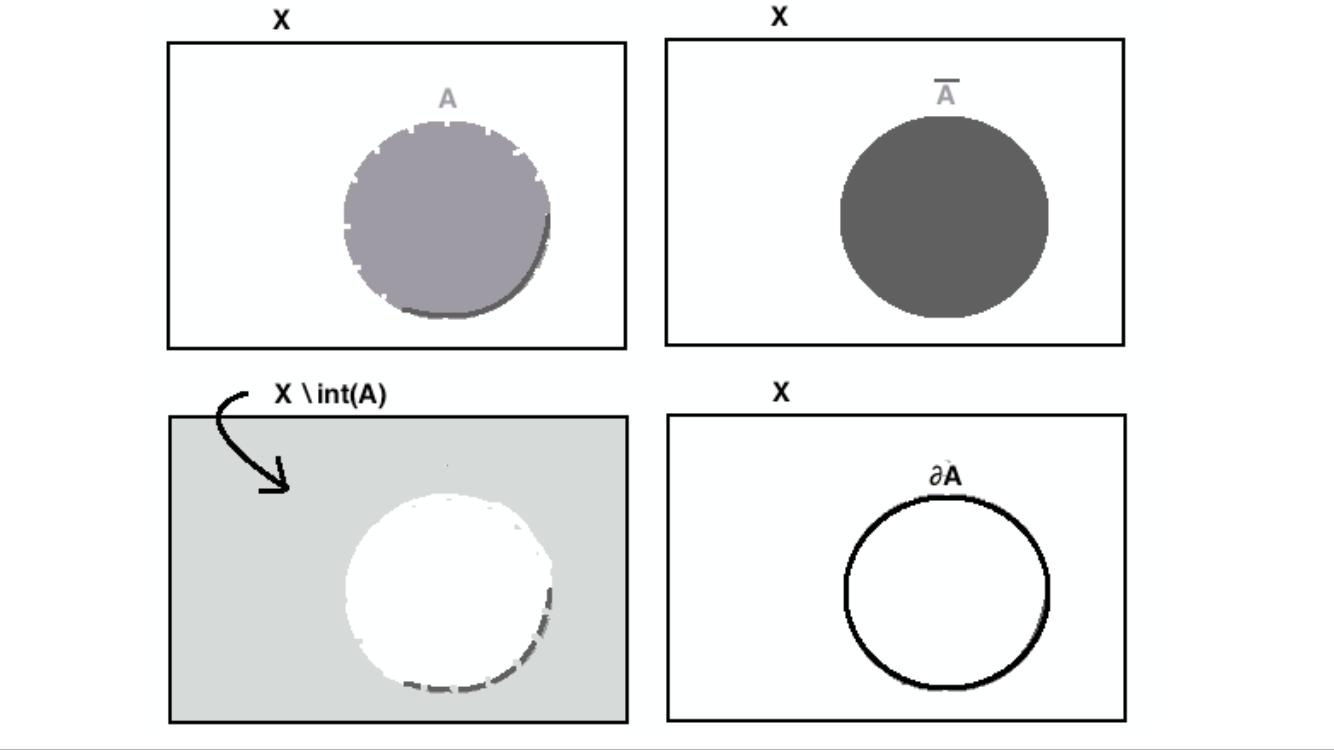
\includegraphics[scale = 0.2]{fotos_topo_1/frontera1.jpeg}
\end{equation}

\begin{coro}
\label{coro:frontera1} Sigui $(X,\tau)$ un espai topològic i sigui $A\subseteq X$. Aleshores $\partial A = \partial (X\setminus A)$.
\end{coro}

\begin{coro}
\label{coro:frontera2} Sigui $(X,\tau)$ un espai topològic i $A\subseteq X$. Aleshores $\partial A$ és tancat.
\end{coro}

Les demostracions d'aquests dos corol·laris no les faig perquè són directes de la definició de frontera (\ref{def:frontera}), del lema (\ref{lema:laclausuradelcomplementarieselcomplementaridelinterior}) i de la proposició (\ref{prop:fronteraa}).

\begin{ej}
\label{ej:frontera1} Sigui $(\mathbb{R},\tau)$ amb la topologia euclidiana. Considerem $A = [0,1)\subseteq \mathbb{R}$. La clausura d'$A$ és $\overline{A} = [0,1]$ i $A^\circ = (0,1)$. Així doncs, $\partial A = \{0,1\}$.
\end{ej}

\begin{ej}
\label{ej:frontera2} Per $B = [0,1)\cup (2,3)\subset\mathbb{R}$ amb la topologia euclidiana, la clausura és $\overline{B} = [0,1]\cup[2,3]$ i l'interior és $B^\circ = (0,1)\cup (2,3)$. Finalment $\partial B = \{0,1,2,3\}$.
\end{ej}

\begin{ej}
\label{ej:frontera3} Sigui $X = \mathbb{R}^3$ amb la topologia euclidiana i considerem $A = [0,1)^2\subseteq \mathbb{R}^2$. Aleshores $A^\circ=(0,1)^2$ i $\overline{A} = [0,1]^2$. Així doncs,
\begin{equation}
    \notag
    \partial A = (\{0\}\times[0,1])\cup(\{1\}\times[0,1])\cup([0,1]\times\{0\})\cup([0,1]\times\{1\}).
\end{equation}
\begin{equation}
    \notag
    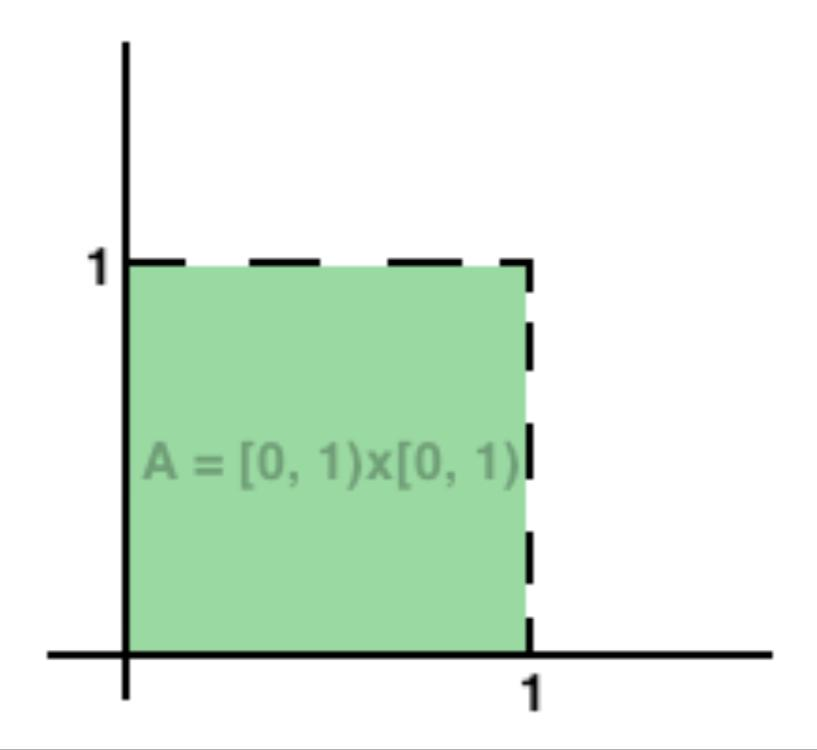
\includegraphics[scale=0.2]{fotos_topo_1/fronteraex3(1).jpeg}
    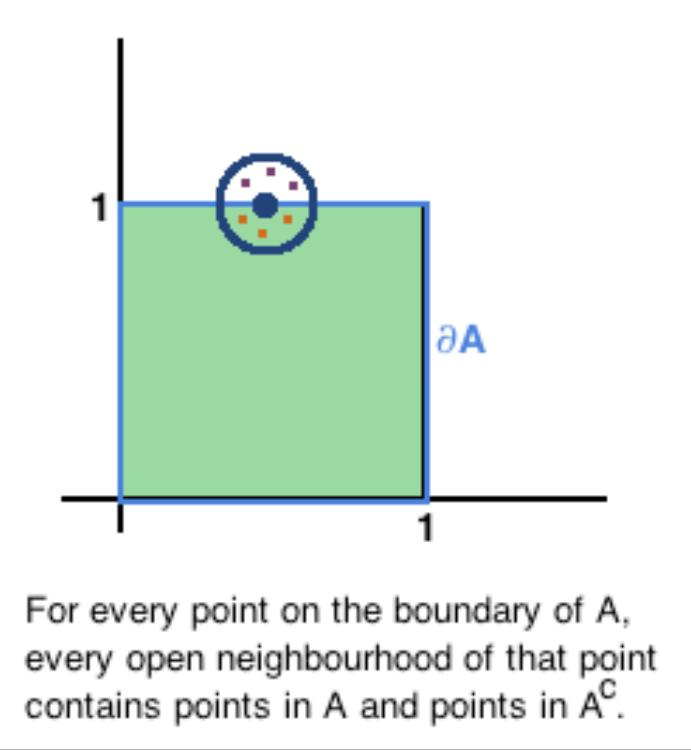
\includegraphics[scale = 0.2]{fotos_topo_1/fronteraex3(2).jpeg}
\end{equation}
\end{ej}

\begin{ej}
\label{ej:frontera4} Sigui $X = \{a,b,c\}$ i $\tau = \{\emptyset,\{a\},\{b,c\},X\}$. Considerem $A = \{a\}$. Què és $\partial A$? Com $A = \{a\}$, $A^c = \{b,c\}$. Podem dir que $A^\circ = \{a\}$ i que $\overline{A} = \{a\}$ ja que si $\{b,c\}$ és obert, $X\setminus\{b,c\} = \{a\}$ és tancat. Així doncs, $\partial A = \emptyset$.
\end{ej}

Aquest últim exemple ens porta a deduir que si un subconjunt és obert i tancat a l'hora, aleshores la seva frontera serà el buit.

\begin{prop}
\label{prop:fronteraclopen} Sigui $(X,\tau)$ un espai topològic i $A\subseteq X$. Aleshores $A$ és obert i tancat a l'hora si i només si $\partial A=\emptyset$
\end{prop}
\begin{proof}
Cap a la dreta, suposem que $A$ és obert i tancat. Aleshores $A^\circ = A$ i $\overline{A} = A$ i com que $A^\circ\subseteq A\subseteq \overline{A}$ obtenim la igualtat $A^\circ=\overline{A}$. Per tant $\partial A = \overline{A}\setminus A^\circ = A\setminus A = \emptyset$. Cap a l'esquerra, suposem que $\partial A = \emptyset$. Aleshores $\partial A = \overline{A}\setminus A^\circ=\emptyset\Rightarrow \overline{A}= A^\circ$ i per tant $A$ és obert i tancat perquè és igual a la seva clausura i al seu interior.
\end{proof}

\begin{coro}
\label{coro:fronteradelbuit} $\partial \emptyset = \emptyset$ i $\partial X = \emptyset$
\end{coro}
\begin{proof}
Com $X$ i $\emptyset$ són sempre oberts i tancats a l'hora, per la proposició (\ref{prop:fronteraclopen}) obtenim el resultat.
\end{proof}

\begin{ej}
\label{ej:frontera5} Sigui $X = \{a,b,c,d\}$ dotat de la topologia
\begin{equation}
    \notag
    \tau = \{\emptyset,\{a\},\{b\},\{a,b\},\{b,d\},\{a,b,d\},X\}. 
\end{equation}
Considerem el conjunt $A = \{a,b,c\}$. Què és $\partial A$?
Com $A = \{a,b,c\}$ tenim $A^c=\{d\}$. 

Els oberts contenint $a$ són $\{a\},\{a,b\}$ i $\{a,b,d\}$ i $X$. Notem que $A^c\cap \{a\} = \emptyset$ i per tant $a\not\in\partial A$. Fem el mateix amb $b$, $c$ i $d$. 

Els oberts contenint $b$ són $\{b\}$, $\{a,b\}$, $\{b,d\}$, $\{a,b,d\}$ i $X$. Notem que $A^c\cap \{b\}=\emptyset$ i per tant $b\not\in\partial A$. 

Prenem ara el punt $c\in X$. Veiem que l'únic obert que el conté és $X$ i $A\cap X\not=\emptyset$ i $A^c\cap X\not=\emptyset$. Per tant, $c\in \partial A$. 

Per últim mirem el punt $d\in X$. Els oberts contenint $d$ són $\{b,d\}$, $\{a,b,d\}$ i $X$. Notem que $A\cap\{b,d\}=\{b\}\not=\emptyset$ i $A^c\cap \{b,d\} = \{d\}\not=\emptyset$. També $A\cap\{a,b,d\}=\{a,b\}\not=\emptyset$ i $A^c\cap\{a,b,d\} = \{d\}\not=\emptyset$. Finalment, $X\cap A\not=\emptyset\not=X\cap A^c$, per tant $d\in\partial A$.

Així doncs, hem trobat que $\partial A = \{c,d\}$.
\end{ej}



\subsection{Propietats}

Sigui $A,B\subseteq X$ on $X$ és un espai topològic. Si $A\subseteq B$, és cert que $\partial A\subseteq \partial B$? La resposta és que no. En el dibuix es veu bastant trivialment:
\begin{equation}
    \notag
    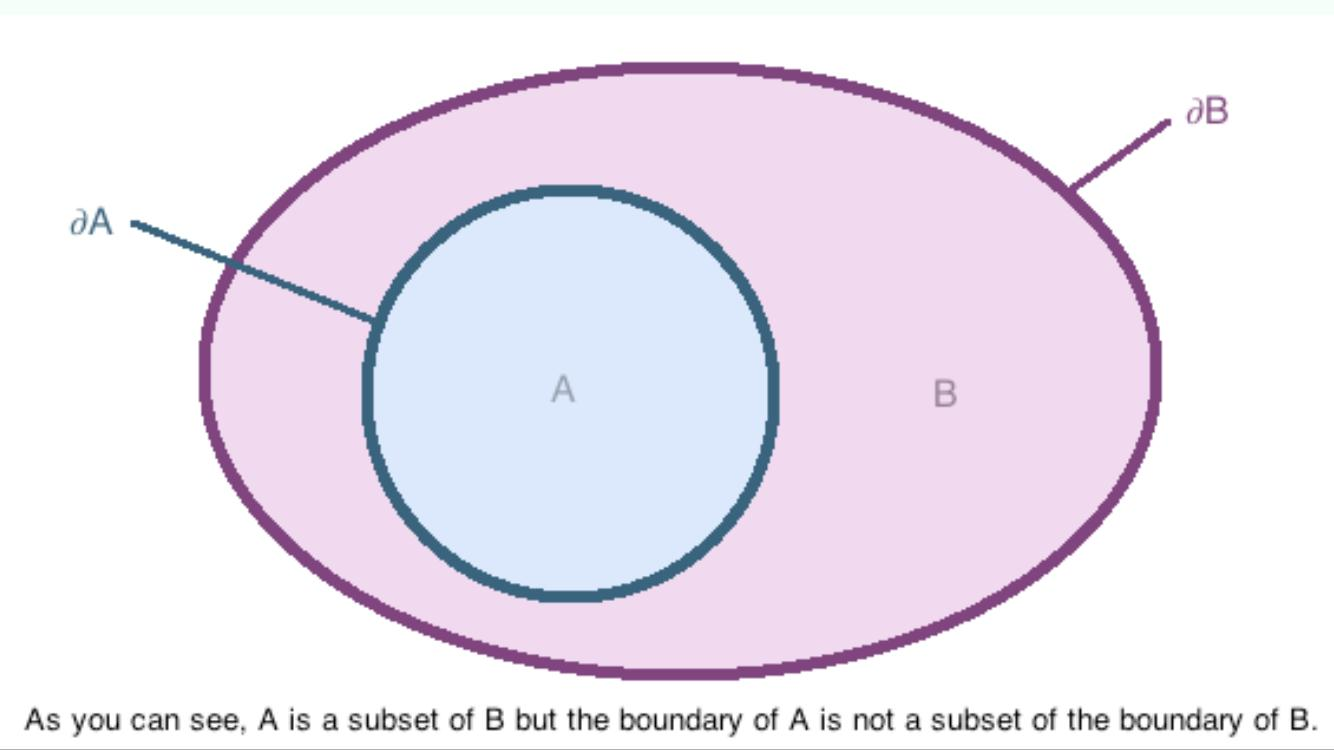
\includegraphics[scale = 0.2]{fotos_topo_1/fronteraprop1.jpeg}
\end{equation}

Per exemple, considerem $(\mathbb{R}^2,\tau)$ amb la topologia euclidiana. Considerem els conjunts $A = \{(x,y)\in\mathbb{R}^2\;:\;x^2+y^2<1\}$ i $B = \{(x,y)\in\mathbb{R}^2\;:\;x^2+y^2<4\}$. Observem que $\partial A = \{(x,y)\in\mathbb{R}^2\;:\;x^2+y^2=1\}$ i $\partial B = \{(x,y)\in\mathbb{R}^2\;:\;x^2+y^2=4\}$. Aleshores $A\subseteq B$ però $\partial A\not\subseteq \partial B$.
\begin{equation}
    \notag
    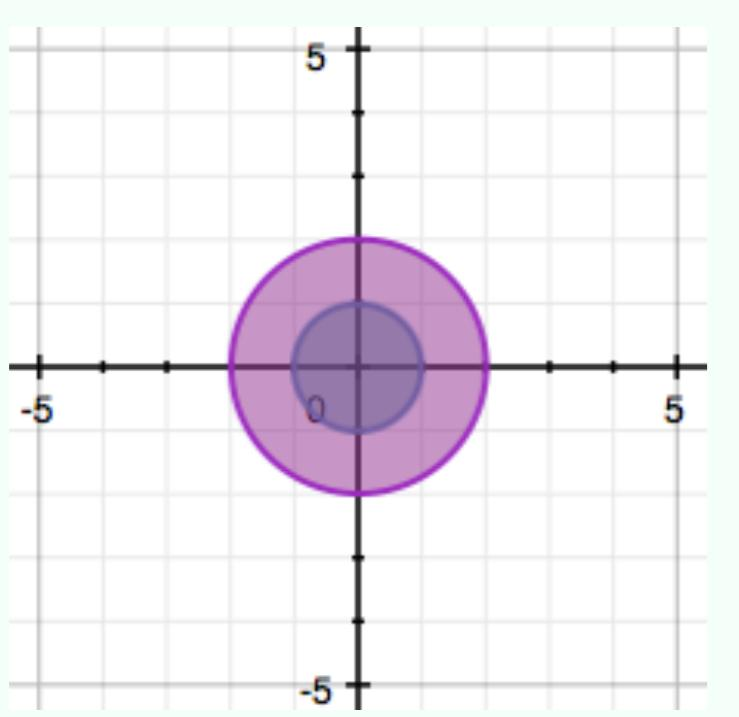
\includegraphics[scale = 0.2]{fotos_topo_1/fronteraprop2.jpeg}
    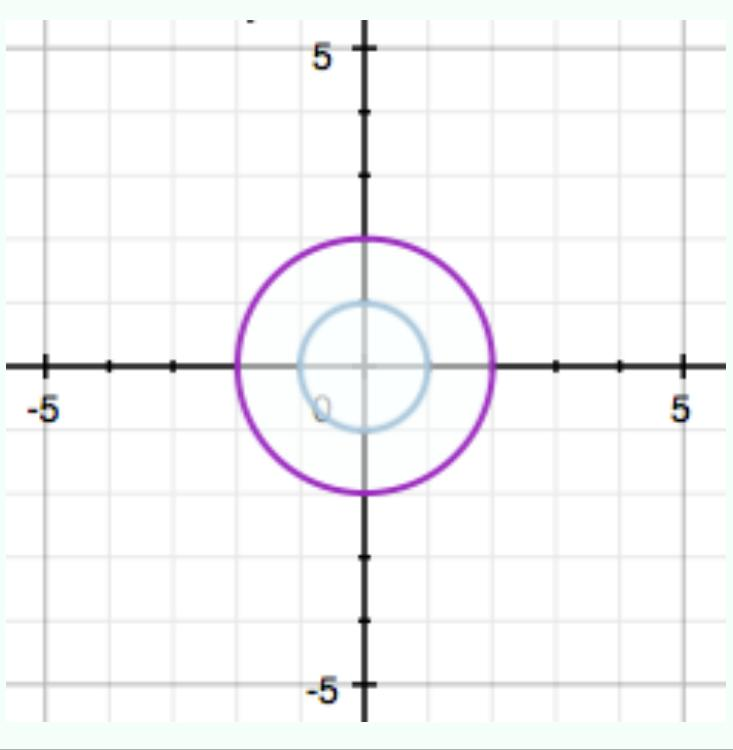
\includegraphics[scale = 0.2]{fotos_topo_1/fronteraprop3.jpeg}
\end{equation}

\begin{prop}
\label{prop:propietat1frontera} Sigui $(X,\tau)$ un espai topològic i $A,B\subseteq X$. Se satisfà $\partial A\cup \partial B\supseteq  \partial (A\cup B)$.
\end{prop}
\begin{equation}
    \notag
    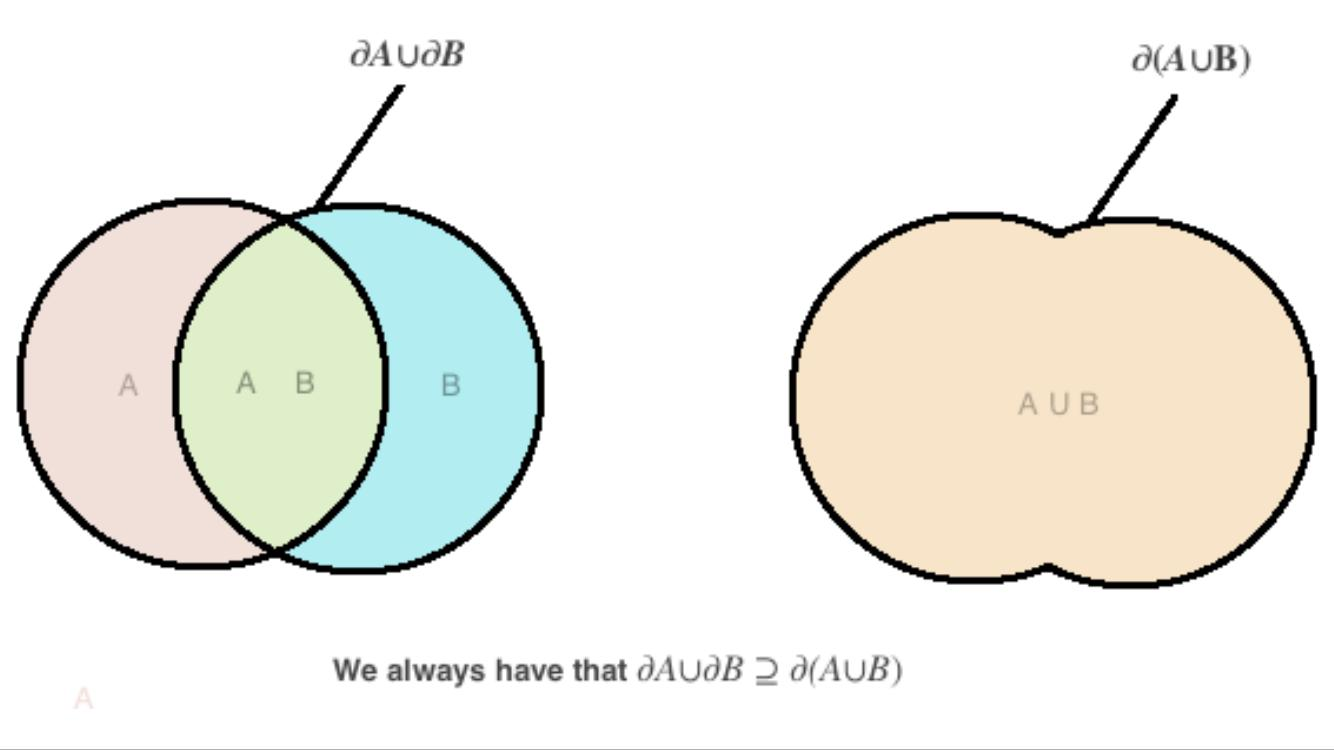
\includegraphics[scale = 0.2]{fotos_topo_1/fronteraprop4.jpeg}
\end{equation}
\begin{proof}
Sigui $x\in\partial (A\cup B)$. Aleshores $x\in (\overline{A\cup B})\setminus(A\cup B)^\circ$. Com $x\in\overline{A\cup B}$, $x\in \overline{A}\cup \overline{B}$ per la proposició (\ref{prop:propietat2clausura}) i per tant $x\in\overline{A}$ o bé $x\in \overline{B}$. Similarment $x\not\in (A\cup B)^\circ$. Per tant $x\not\in A^\circ\cup B^\circ$ per (\ref{prop:propietat2interior}) i per tant $x\not\in A^\circ$ o bé $x\not\in B^\circ$. Combinant aquests fets:
\begin{equation}
    \notag
    x\in (\overline{A}\setminus A^\circ)\cup (\overline{B}\setminus B^\circ) = \partial A\cup \partial B
\end{equation}
com volíem veure.
\end{proof}

Atenció perquè no és cert que $\partial A\cap \partial B\subseteq \partial (A\cap B)$. Un contraexemple és si $X = \mathbb{R}$ i $\tau$ és la topologia euclidiana, prenem $A = [0,1)$ i $B=(1,2)$. Aleshores $A\cap B = \emptyset$, ergo $\partial (A\cap B)= \partial \emptyset = \emptyset$ per (\ref{coro:fronteradelbuit}). D'altra banda, però, $\partial A = \{0,1\}$ i $\partial B = \{1,2\}$ així que $\partial A\cap \partial B = \{1\}\not\subseteq\emptyset$.

Tampoc és cert que $\partial A\cup \partial B\subseteq \partial (A\cup B)$. Un contraexemple pot ser el mateix que l'anterior.

\begin{prop}
\label{prop:propietat2frontera} Sigui $(X,\tau)$ un espai topològic i sigui $A\subseteq X$. Aleshores $A$ és obert si i només si $A\cap \partial A=\emptyset$.
\end{prop}
\begin{proof}
Suposem que $A$ és obert. Aleshores $A = A^\circ$. Observem que si $x\in\partial A$, aleshores $x\in \overline{A}\setminus A^\circ$ i per tant $x\not\in A^\circ = A$. Així $\partial A\cap A=\emptyset$. Recíprocament, suposem que $\partial A\cap A =\emptyset$. Sigui $x\in A$. Aleshores $x\not\in\partial A$. Així, $x\not\in \overline{A}\setminus A^\circ$ i aleshores $x\in A^\circ$, ergo $A = A^\circ$.
\end{proof}

\begin{prop}
\label{prop:propietat3frontera} Sigui $(X,\tau)$ un espai topològic i sigui $A\subseteq X$. Aleshores $A$ és tancat, si i només si $\partial A\subseteq A$.
\end{prop}
\begin{proof}
Sigui $A$ tancat. Aleshores $X\setminus A$ és obert i per la proposició anterior (\ref{prop:propietat2frontera}) obtenim que $(X\setminus A)\cap \partial (X\setminus A) = \emptyset$. Però per (\ref{coro:frontera2}) $\partial (X\setminus A) = \partial A$. Així $X\setminus A$ i $\partial A$ són disjunts i aleshores $\partial A\subseteq A$. Recíprocament, si $\partial A\subseteq A$, aleshores $(X\setminus A)\cap \partial A = \emptyset$. Equivalentment $(X\setminus A)\cap \partial (X\setminus A)=\emptyset$. Aleshores $X\setminus A$ és obert i per tant $A$ és tancat.
\end{proof}




\section{Conjunt dens en un espai topològic}
\begin{defi}
[Dens]\label{def:dens}\index{Dens}\index{Conjunt dens} Sigui $(X,\tau)$ un espai topològic. El conjunt $A\subseteq X$ es diu \textit{dens} en $X$ si la intersecció de tot obert no buit amb $A$ és no buida. És a dir, si $\forall U\in\tau\setminus\{\emptyset\}$, $A\cap U\not=\emptyset$.
\end{defi}

Donada una topologia $\tau$ en $X$, és important notar que $X$ és dens en $X$, ja que tot $U\in\tau\setminus\{\emptyset\}$ tal que $U\subseteq X$ compleix que $U\cap X = U\not=\emptyset$.

\begin{ter}[Exemple]
\label{ej:qesdensar} Considerem l'espai topològic $(\mathbb{R},\tau)$, on $\tau$ és la topologia usual. Aleshores, el conjunt dels racionals $\mathbb{Q}$ és dens en $\mathbb{R}$.
\end{ter}
\begin{proof}
Suposem que no ho és: suposem que $\exists U\in\tau\setminus\{\emptyset\}$ tal que $\mathbb{Q}\cap U = \emptyset$. Com $U\in\tau$, tenim que $(a,b)\in U$, per a alguns $a,b\in\mathbb{R}$, $a<b$, ja que $U$ és unió d'intervals oberts del tipus $(a,b)\subset\mathbb{R}$ (perquè és unió d'elements de la base, veure (\ref{def:base})). Suposant $\mathbb{Q}\cap U = \emptyset$, tenim que
\begin{equation}
    \notag
    \mathbb{Q}\cap U \Longrightarrow \mathbb{Q}\cap (a,b) = \emptyset.
\end{equation}
Això implica que l'interval $(a,b)$ no conté cap nombre racional, cosa que sabem és impossible perquè $\forall a,b\in\mathbb{R}$, $a<b$, sempre existeix un racional $q\in\mathbb{Q}$ tal que $a<q<b$. Per tant això és una contradicció i $U\cap\mathbb{Q}\not=\emptyset$, $\forall U\in\tau\setminus\{\emptyset\}$.
\end{proof}

\begin{prop}
\label{prop:dens} Sigui $(X,\tau)$ un espai topològic i $A\subset X$. Aleshores, $A$ és dens si, i només si, $\overline{A}=X$.
\end{prop}

\begin{ej}
\label{ej:dens2} Considerem l'espai topològic $(\mathbb{R}^2,\tau)$, on $\tau$ és la topologia usual dels discs oberts. Considerem
\begin{equation}
    \notag
    A = \{(x,y)\in\mathbb{R}^2\;:\;x\in\mathbb{N},y\in\mathbb{R}\}\subseteq\mathbb{R}^2.
\end{equation}
Veiem que aquest conjunt no és dens. Hem de trobar un obert $U$ de $\mathbb{R}^2$ per al qual $A\cap U = \emptyset$. Considerem el següent disc obert en $\mathbb{R}^2$:
\begin{equation}
    \notag
    U = \{(x,y)\in\mathbb{R}^2\;:\;(x-1/2)^2+y^2<1/4\} .
\end{equation}
Aquest disc està centrat al punt $(1/2,0)$ i té radi $1/2$. No interseca amb $A$ (no hi ha cap punt a $U$ que tingui la primera component natural), per tant és un contraexemple.
\end{ej}












\end{document}
